%% ------------------------------------------------------------------------- %%
\chapter{Conceitos}
\label{cap:conceitos}

%% ------------------------------------------------------------------------- %%
\section{Imagem Digital}\index{Imagem Digital}
\label{sec:imagemDigital}

  Uma imagem digitial 3D I é representada por um vetor tridimensional, onde cada
posição, chamada de \textit{voxel}, é acessada pela função
\begin{align}\label{eq:defImagem}
    I(x,y,z) = i
\end{align}
  para $x, y, z \in \mathbb{N}$.

%% ------------------------------------------------------------------------- %%
\section{Registro}\index{Registro}
\label{sec:fundamentos}

  O registro tem como objetivo alinhar uma imagem, a imagem alvo (\textit{IA}),
geométricamente à outra imagem, a imagem referência (\textit{IR}). Esse
alinhamento é realizado encontrando correspondências entre pontos das duas imagens,
que são usadas para encontrar uma função de deformação que mapeia todos os
pontos da imagem alvo à pontos da imagem referência.

O registro possibilita, por exemplo, a união de informação de imagens de
diferentes modalidades (figura \ref{fig:multiModal}), o reconhecimento de
objetos dentro de cenas, reconhecimento de diferenças entre imagens e
a recuperação de pequenas deformações sofridas por uma imagem (figura
\ref{fig:regExplicacao}).

Os algoritmos de registro podem ser divididos, com algumas resalvas, em cinco
passos gerais:
\begin{enumerate}
    \item Pré-processamento;
    \item Detecção de características;
    \item Correspondência de características;
    \item Estimativa da função de transformação;
    \item Reamostragem da imagem Alvo.
\end{enumerate} % TODO: Colocar o diagrama aqui %

%% ------------------------------------------------------------------------- %%
\subsection{Pré-processamento}
  O objetivo do pré-processamento é a normalização dos dados de entrada. Essa
normalização é realizada por dois motivos diferentes. O primeiro é para corrigir
divergencias em caracteristicas das imagens, como diferentes escalas, intensidade
de iluminação ou presença de ruido. Tais caracteristicas devem ser equalizadas
entre todas as entradas afim de uniformizar os próximos passos do registro.

Vários algoritmos renomados dentro da área de visão computacional são aplicados
nessa etapa com o propósito de normalizar as entradas. Por exemplo, temos
as seguintes operações:

\begin{description}
    \item [\textit{Reamostragem}] Algoritmos utilizados para reamostrar a imagem,
          modificando sua escala. Exemplos: Interpolação linear e quadrática.
    \item [\textit{Suavização}] Algoritmos utilizados para a remoção de ruido da
          imagem. Exemplos: Filtros passa baixa, passa alta e gaussiano.
    \item [\textit{Mudança de Contraste}] Algoritmos utilizados para equalizar
          a distribuição do histogramas em imagens. Exemplos: Equlização de histograma.
          \ref{fig:equalization}
\end{description}

\begin{figure}[H]
    \centering
    \begin{subfigure}[t]{0.3\textwidth}
      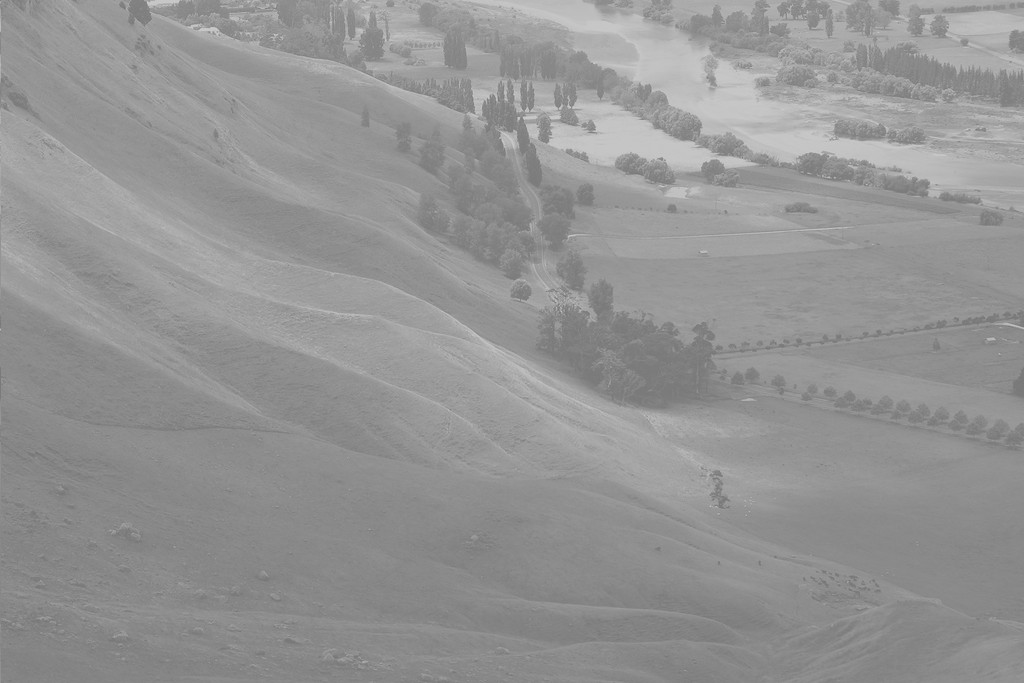
\includegraphics[width=\textwidth]{figuras/Unequalized.jpg}
      \subcaption*{(a)}
      \label{fig:unequalizedImage}
    \end{subfigure}
    \begin{subfigure}[t]{0.3\textwidth}
      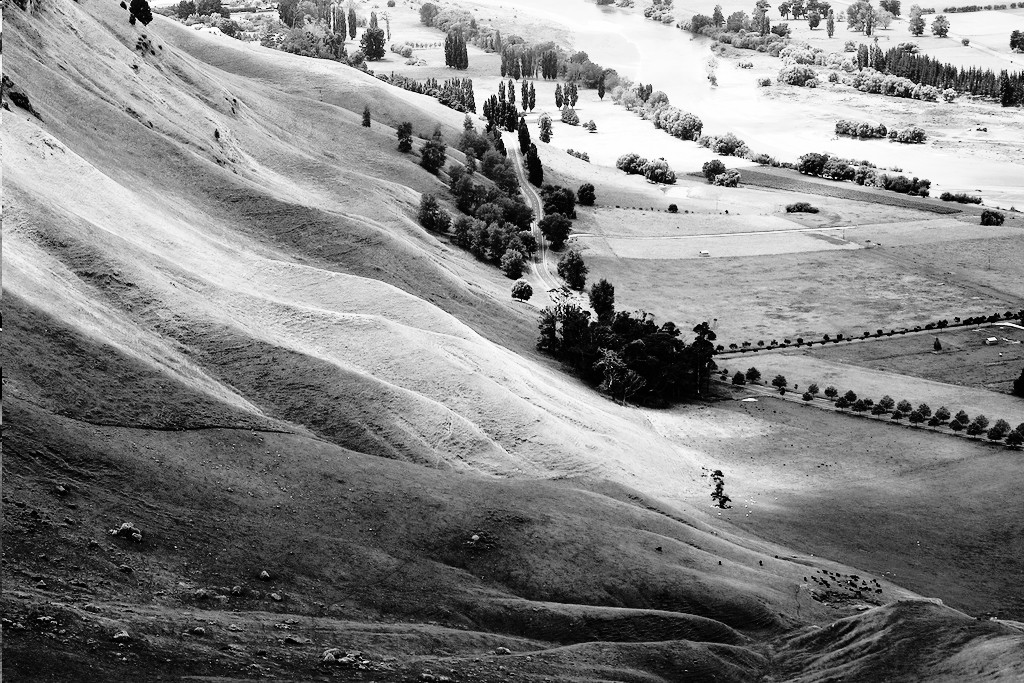
\includegraphics[width=\textwidth]{figuras/Equalized.jpg}
      \subcaption*{(b)}
      \label{fig:equalizedImage}
    \end{subfigure}
    \source{https://en.wikipedia.org/wiki/Histogram\_equalization}
    \caption{Exemplo do uso da equalização de histograma para realçar o terreno
            na imagem. (a) Imagem não equalizada. (b) Imagem equalizada.}
    \label{fig:equalization}
\end{figure}


O segundo motivo pelo qual o pré-processamento é utilizado é a extração de
informação das imagens, ou segmentação. O próximo passo do registro, a detecção
de características, dita quais serão as informações extraidas neste passo. Como
exemplo de segmentação, temos:

\begin{description}
    \item [\textit{Limiarização}] Processo básico de segmentação, onde voxels
          tem sua intensidade modificada caso a mesma falhe na checagem com um
          certo valor limite. Exemplos: Limiarização por histograma, por cor ou
          \textit{clusterização}.
    \item [\textit{Detecção de borda}] Uilizados para realçar bordas encontradas
          em imagens. Uma borda é definida como uma região com uma grande
          variação de intensidade. Exemplos: Canny, Laplacian. \ref{fig:edgeDetection}
\end{description}

\begin{figure}[H]
    \centering
    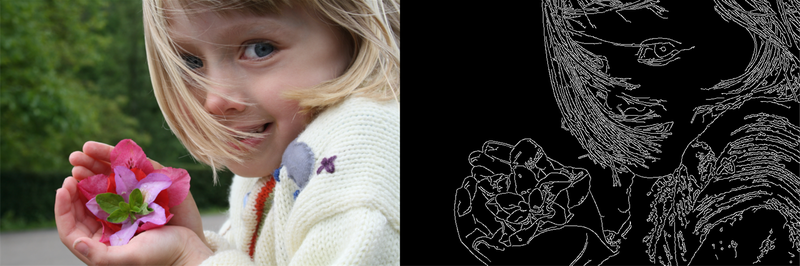
\includegraphics[width=0.8\textwidth]{figuras/canny.png}
    \source{https://en.wikipedia.org/wiki/Canny\_edge\_detector}
    \caption{Resultado do algoritmo de detecção de bordas Canny. A imagem à
    esquerda é a imagem de entrada, e a imagem à direita contém as bordas
    encontradas pelo Canny.}
    \label{fig:edgeDetection}
\end{figure}

\begin{figure}[H]
  \centering
  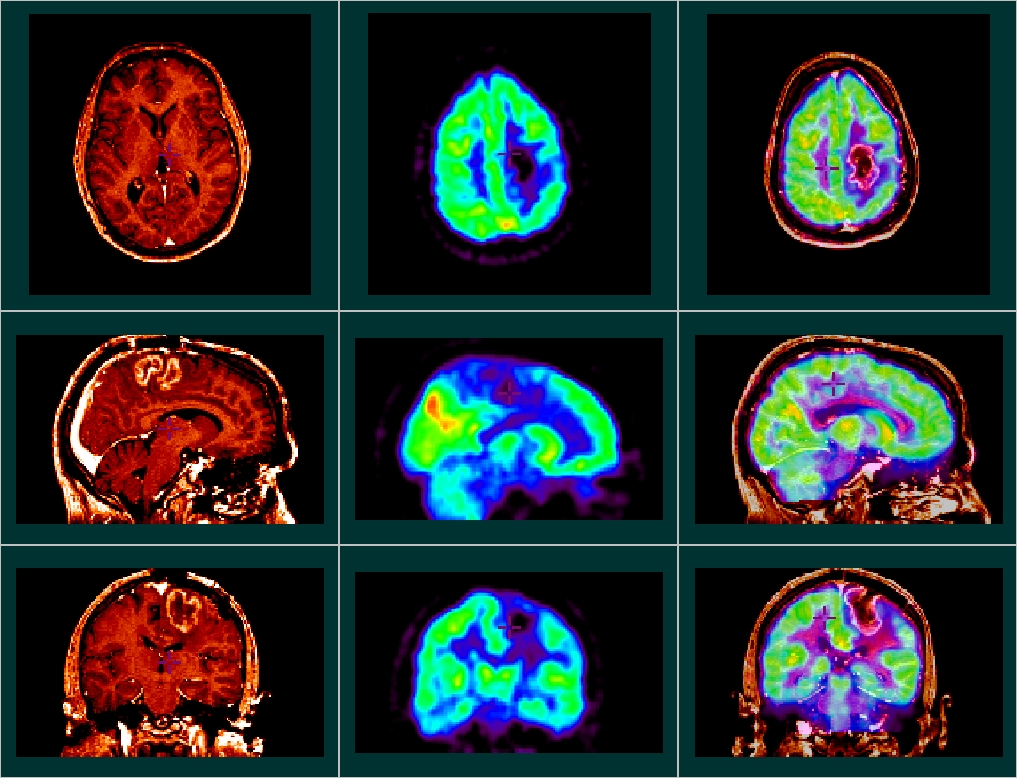
\includegraphics[width=0.8\textwidth]{figuras/multiModal.jpg}
  \caption{Exemplo de registro multimodal. Nas duas primeiras colunas temos
  imagens construidas a partir de, respectivamente, MRI e PET. Na terceira
  coluna temos o resultado do registro.}
  \source{http://cecs.wright.edu/~agoshtas/nih96.html}
  \label{fig:multiModal}
\end{figure}

\begin{figure}[H]
    \centering
    \begin{subfigure}[t]{0.3\textwidth}
      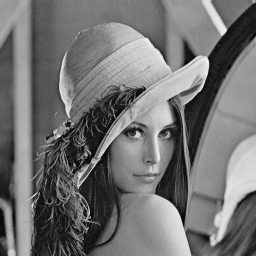
\includegraphics[width=\textwidth]{figuras/static.png}
      \subcaption*{(a)}
      \label{fig:ref-image}
    \end{subfigure}
    \begin{subfigure}[t]{0.3\textwidth}
      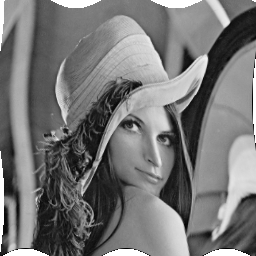
\includegraphics[width=\textwidth]{figuras/lenaMoving.png}
      \subcaption*{(b)}
      \label{fig:sin-image}
    \end{subfigure} \\
    \begin{subfigure}[t]{0.64\textwidth}
      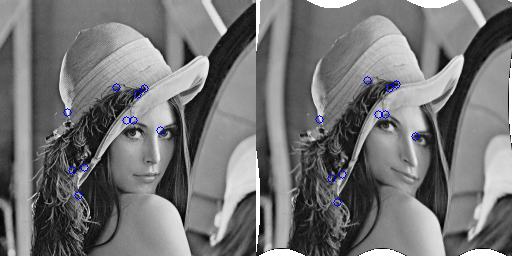
\includegraphics[width=\textwidth]{figuras/Features.png}
      \subcaption*{(c)}
      \label{fig:dist-image}
    \end{subfigure} \\
    \begin{subfigure}[t]{0.3\textwidth}
      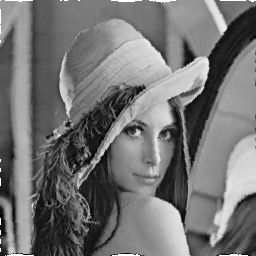
\includegraphics[width=\textwidth]{figuras/lenaRegistrada.png}
      \subcaption*{(f)}
      \label{fig:lenaRegistrada}
    \end{subfigure}
    \caption{Exemplo do uso do registro para retirada de uma deformação artificial.
             (a) Imagem Referência. (b) Imagem Alvo. (c) Detecção de características.
             (d) Correspondência de características. (e) Estimativa da função de transformação.
             (f) Reamostragem da imagem Alvo.}
    \label{fig:regExplicacao}
\end{figure}


%% ------------------------------------------------------------------------- %%
\subsection{Detecção de características}\index{Detecção de características}
\label{sec:dec_corr_carac}

    Com as imagens já preprocessadas, o primeiro passo para um algoritmo de registro é a localização de estruturas de
destaque na cena ou objeto dentro das imagens. Essas estruturas são nomeadas de características, e são construídas a
partir de um conjunto de pixels. Características devem ser facilmente identificadas, independente de variações na
aquisição das fotografias, como mudanças na angulação ou perspectiva. Elas são separadas em 3 grupos, a seguir:

\textbf{Baseadas em Região} - As características de Região são áreas de uma imagem que apresentam uma diferença
significativa de contraste em relação a áreas vizinhas. Normalmente são representadas por um
conjunto conexo de pixels ou utilizando um \textit{template} de formato retangular ou circular centrado no centro de
massa da Região. Lagos, florestas ou regiões urbanas são exemplos desse tipo de
característica.

\textbf{Baseadas em Retas} - Essas características são definidas como a interface entre duas regiões de uma
imagem, comumente chamadas de bordas. Exemplos comuns são ruas, rios ou o litoral, onde
podemos claramente visualizar a diferença de intensidade, por exemplo, do mar e da areia. Métodos clássicos de detecção
de bordas como o Canny ou o filtro Laplaciano são usados para identificar essas características.

\textbf{Baseadas em Ponto} - São pontos que conseguem representar a região na qual se encontram atráves de alguma
propriedade invariável a mudanças na cena, como intersecções de linhas ou pontos de máxima curvatura. Algoritmos para
identificação de pontos utilizam técnicas mais avançadas, dada a dificuldade de encontrá-los. Os mais básicos encontram
as intersecções de linhas enquanto os mais avançados buscam centroides de regiões ou o máximo local de uma
\textit{wavelet}.

  Encontrar características em imagens é um passo não só de registro de imagens, mas em reconhecimento de padrões,
reconstrução de modelos 3D e outras áreas. Dada essa importância, vários algoritmos foram desenvolvidos com o passar dos
anos para resolver de maneira rápida e eficiente a detecção de características. Falaremos sobre dois métodos firmados
no meio científico, o \textit{Scale Invariant Feature Transform} (SIFT) , introduzido por \cite{lowe2004distinctive}, e
o \textit{Speeded Up Robust Features} (SURF), desenvolvido por \cite{bay2008speeded}. Como esse métodos fazem tanto a
captura das característica quanto a correspondência entre elas falamos sobre eles na próxima seção.

%% ------------------------------------------------------------------------- %%
\subsection{Correspondência de características}\index{Correspondência de características}

    Com as características de cada uma das imagens encontradas, o próximo passo é realizar a correspondência entre elas.
A função desse passo é encontrar a correspondência entre pontos da imagem Referência para a imagem Alvo, ou vice-versa.
O processo pode ser realizado tanto escolhendo ponto a ponto da imagem Referência e procurando o ponto com maior valor
de proximidade entre os pontos da imagem Alvo, quanto utilizando métodos estatísticos para determinar quais pontos são
correspondentes entre as duas imagens. É importante que esse passo consiga identificar pontos físicos, com coordenadas,
em cada par de características, para que uma primeira estimativa dos parâmetros da função de transformação possa ser
utilizada como ponto de partida para o próximo passo.

    A primeira solução a ser apresentada, a \textbf{Baseada em Área}, mescla o passo de Detecção com o de
Correspondência. Esse método utiliza duas janelas, uma em cada imagem, com formato retangular ou circular, aplicando
métricas em cada uma das janelas com a finalidade de calcular a relação entre as janelas. O algoritmo segue realizando
esse cálculo para todas as combinações possíveis de janelas entre as duas imagens, e sempre que um máximo é encontrado
o centro das janelas são usados para marcar a correspondência. Várias métricas podem ser utilizadas, como a
Correlação entre as intensidades das janelas, o estudo do espectro da transformada de \textit{Fourier} das janelas ou
o cálculo da informação mútua entre elas.

    A descoberta de correspondência entre características \textbf{Baseadas em Região} é feita utilizando, principalmente, duas
técnicas. A primeira, mais simples na sua ideia, é parear regiões da imagem Referência com a região da imagem Alvo a
qual tenha o contorno mais parecido possível. Os métodos que fazem esse pareamento devem ser capazes de encontrar os
pares mesmo que eles tenham sofrido rotações ou mudança de escala. Descritores de Fourier e representações matriciais
das regiões são exemplos de métodos usados para realizar a correspondência entre características de região.

    Os métodos para encontrar correspondências entre \textbf{Baseada em Retas} tem as mesmas restrições que os
de Região, ou seja, devem conseguir realizar o pareamento de linhas que sofreram rotação, mudança de escala ou
translação. O primeiro passo de um algoritmo é comparar as retas da imagem Referência com todas as possíveis rotações
de todas as retas da imagem Alvo. Quando um possível par é encontrado, um valor de correspondência é calculado,
utilizando um peso maior para a direção da reta, algo que não sofre tanta influência de ruído, e um peso menor para
atributos como comprimento e largura, que são influenciados pelo ruído. O algoritmo ainda deve ser capaz de parear mais
de duas retas por vez, dada a possibilidade de uma reta em uma das imagens ser representada por duas retas na outra
imagem.

    Por fim, as correspondências entre \textbf{Características de Ponto} podem ser encontradas utilizando-se várias
técnicas distintas. Como o número e o agrupamento de pontos geralmente não muda tanto com rotações e translações de
imagens, métodos de \textit{Clustering} são usados para parear pontos. Os \textit{Clusters} são montados com base na
proximidade dos parâmetros de uma transformação que leve pontos da imagem Alvo para pontos da imagem Referência. Outro
método define as características através de descritores invariantes que podem obedecer a 4 regras: \textbf{Invariância},
características correspondentes devem ter os mesmos descritores; \textbf{Unicidade}, características diferentes devem
ter descritores diferentes; \textbf{Estabilidade}, os descritores devem deformar de maneira proporcional a deformação
aplicada na imagem; e \textbf{Independência}, se o descritor for representado por um vetor, seus componentes devem ser
independentes. O que define um descritor deve ser decidido caso a caso. O modelo mais simples usado é a própria
intensidade do pixel, e a intensidade de seus vizinhos. Outros descritores válidos são ângulos entre correspondências
vizinhas ou a distribuição espacial dos vizinhos.

  Abaixo falamos sobre o \textit{Scale Invariant Feature Transform} e o \textit{Speeded Up Robust Features}, que são
métodos que fazem tanto a captura quanto a correspondência de características.

\subsubsection{Scale Invariant Feature Transform (SIFT)}
  O SIFT cria, para cada característica, um vetor de propriedades invariáveis com rotações, mudanças de escala e
translações, e parcialmente invariáveis com mudanças de projeção e iluminação. O primeiro passo do algoritmo é encontrar
posições, que ele chama de \textbf{chave}, que obedeçam as propriedades acima. Para isso ele faz uma busca no espaço
de escala de uma imagem, procurando pelo máximo ou minimo da diferença de Gaussianas nesse espaço.

  O espaço de escala de uma imagem é criado construindo uma piramide de reamostragens de uma imagem. Na base temos a
imagem original e em cada andar da piramide se encontra uma versão reamostrada da imagem. Antes de reamostrar a próxima
imagem da piramide, o SIFT aplica 2 vezes um filtro Gaussiano com desvio padrão $\sigma = \sqrt{2}$ a imagem atual,
criando mais duas imagens, que chamaremos de $A$ e $B$, respectivamente. A reamostragem para criar o próximo patamar da
piramide é criado aplicando uma interpolação bilinear com espaçamento de $1.5$ pixels a imagem $B$ do patamar atual.

  A busca pelos mínimos ou máximos da diferença de Gaussianas é feita de uma maneira não direta, com fim de otimizar
o cálculo. Primeiro, cada pixel da imagem é comparado com seus 8 vizinhos. Se ele é um minimo ou máximo então calculamos
sua projeção na imagem abaixo, lembrando da reamostragem de $1.5$ pixels. Se ele continua sendo menor ou maior que sua
projeção e os 8 vizinhos da projeção, o processo é repetido para a imagem acima. Os pixels que passarem por essas
etapas são os pixels \textbf{chave}.

  Com os pontos \textbf{chave} encontrados, o algoritmo agora encontra uma orientação e magnitude para eles. Elas são
obtidas calculando o gradiente da imagem $A$ em cada nível da piramide e obtendo a orientação e magnitude deles. Para
tornar a magnitude parcialmente invariável em relação a mudanças de iluminação ela é limiarizada em $0.1$ vezes o valor
da maior magnitude em um nível. A orientação é determinada utilizando um histograma criado a partir de uma Gaussiana
com desvio padrão três vezes maior que o usado no filtro da imagem $A$. Após um processo de suavização no histograma,
seu máximo é escolhido como orientação para o pixel \textbf{chave}.

  Agora o algoritmo irá determinar o vetor descritor para cada ponto \textbf{chave}. Para tal, o algoritmo observa todos
os pixels em uma vizinhança $16 \times 16$ ao redor de cada \textbf{chave}, separando essa vizinhança em 8 menores de $4 \times 4$ pixels.
Para cada vizinhança um histograma de 8 posições de orientações é criada e preenchida utilizando como base uma Gaussiana
com desvio padrão $1.5$ vezes maior que o desvio padrão utilizado para criar a imagem atual. Então, cada uma das 16
vizinhanças irão contribuir com seu histograma de 8 posições, criando um vetor de 128 posições que será utilizado
para descrever o ponto \textbf{chave} em questão.

  A busca de correspondência pode ser feita usando uma busca exaustiva entre todas as características das duas imagens,
porém o autor utiliza uma árvore binária multidimensional de busca (\textit{k-d tree}), populando ela com as
características de uma das imagens e utilizando ela para buscar a característica mais próxima dentre todas as possíveis.

\subsubsection{Speeded Up Robust Features (SURF)}

  O SURF diminui o número de invariáveis que o SIFT utiliza, garantindo somente a invariância em rotações e mudanças de
escala. Ele é separado em três passos: No primeiro, pontos de interesse na imagem são encontrados, normalmente são
cantos, borrões ou junções em T; Depois, um vetor é construído para representar a vizinhança desse ponto; Por fim, a
correspondência de pontos de diferentes imagens é feita.

  O SURF utiliza o determinante da matriz Hessiana para detectar se um ponto $\mathtt{x} = (x, y)$ é um ponto de
interesse:

\begin{align}\label{eq:hessian}
    \mathcal{H}(\mathtt{x}, \sigma) =
      \begin{bmatrix}
        L_{xx}(\mathtt{x}, \sigma) & L_{xy}(\mathtt{x}, \sigma) \\
        L_{xy}(\mathtt{x}, \sigma) & L_{yy}(\mathtt{x}, \sigma)
      \end{bmatrix}
\end{align}

  Onde $L_{xx}(\mathtt{x}, \sigma)$ é a convolução da Gaussiana de segundo grau ($ \frac{\delta^2}{\delta x^2} g(\sigma) $)
no ponto $\mathtt{x}$, e $L_{xy}(\mathtt{x}, \sigma), L_{yy}(\mathtt{x}, \sigma)$ nas outras direções possíveis. Para
cada ponto o determinante da matriz da equação \ref{eq:hessian} é calculada, e uma nova imagem é montada com o resultado.
Porém a utilização das derivadas Gaussiana de segunda ordem leva a perda de repetibilidade, ou seja, encontrar a mesma
característica em imagens com diferença de rotação ou escala. Os autores, então, optam pela utilização de uma aproximação
de uma Gaussiana, chamada de filtro caixa, descrito na imagem \ref{fig:box}.

\begin{figure}[H]
    \centering
    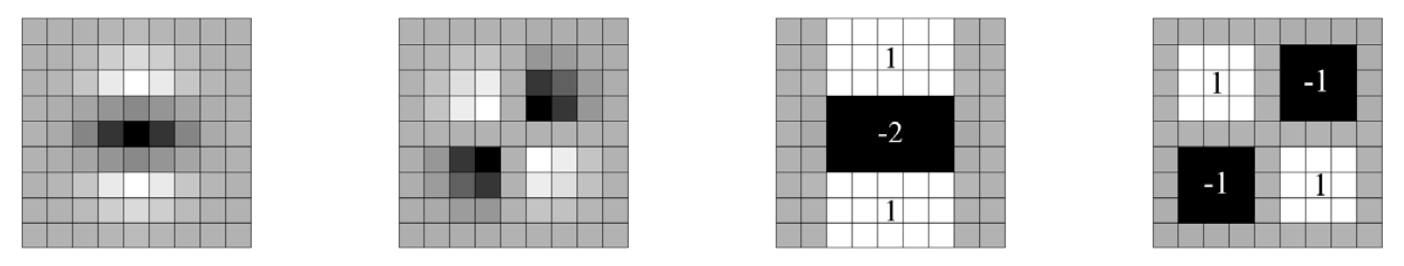
\includegraphics[width=1\textwidth]{figuras/boxFilter.png}
    \caption{As duas primeiras imagens mostram a aplicação da primeira e segunda derivada de uma Gaussiana,
             respectivamente. As duas últimas imagens mostram o filtro caixa. \cite{surfHolroyd}.}
    \label{fig:box}
\end{figure}

  A utilização do filtro caixa em conjunto com as imagens integrais, que representam em cada um de seus pontos a soma
dos pixels do retângulo que vai da origem até o ponto em questão, torna a construção das piramides que representam o
espaço de escala trivial. Ao invés de reamostrar a imagem a cada passo da piramide, basta aumentar o tamanho do filtro
caixa e aplicá-lo diretamente na imagem integral para obter todos os níveis da piramide. Com a piramide de imagens
Hessianas construída, o algoritmo busca numa vizinhança $3 \times 3 \times 3$ os máximos locais para encontrar os
pontos de interesse.

  Para encontrar a orientação dos pontos de interesse, o SURF define uma vizinhança circular de tamanho variado, com
relação ao nível em que a imagem se encontra na piramide. Para cada dimensão da imagem as \textit{wavelets de Haar} são
calculadas, afim de determinar a direção preferencial. Todos os resultados são colocados em um plano $x \times y$, e
todos os valores dentro de todas as janelas de tamanho $\frac{\pi}{3}$ são somados. A direção correspondente a maior
janela é escolhida. Para construir o vetor de descritores uma vizinhança quadrada de tamanho proporcional a escala é
utilizada, sendo subdividida em janelas de tamanho $4 \times 4$. Para cada subjanela uma \textit{wavelets de Haar} é
calculada, e um vetor de 4 dimensões é montado. As duas primeiras dimensões do vetor são construídas usando a soma de
todos os \textit{wavelets de Haar} nas duas dimensões. As duas últimas dimensões são construídas utilizando a soma do
valor absoluto dos \textit{wavelets de Haar}, trazendo informações sobre a polaridade da mudança de contraste.

  Com os descritores construídos, o SURF utiliza um método parecido com o SIFT para realizar a correspondência de
características, utilizando uma árvore binária multidimensional de busca (\textit{k-d tree}), adicionando uma dimensão a
mais quando comparado ao SIFT. O SURF utiliza o traço da matriz Hessiana, que contém informação sobre o contraste da
característica em relação ao fundo no qual ela se encontra.

\subsubsection{Aceleração na Correspondência de Características}

    Podemos separar os algoritmos de correspondências em dois tipos com base no estilo com que eles fazem a busca de
correspondências. O primeiro tipo escolhe uma correspondência na imagem Referência e realiza uma busca em largura por
todas as correspondências da imagem Alvo, buscando aquela com maior relação com a da imagem Referência. Esse processo
pode ser facilmente acelerado utilizando uma paralelização com todas as correspondências da imagem Referência. Já o
outro tipo realiza uma busca entre as relações das características e encontra os pares de maneira iterativa. A
aceleração desse passo depende totalmente da sua implementação.

    O modelo \textit{MapReduce} apresenta uma outra alternativa para acelerar esse passo e o anterior. Ele foi
desenvolvido por \cite{dean2008mapreduce} e pela Google. O modelo \textit{MapReduce} foi desenvolvido para realizar
processamento em lote de um número gigantesco de dados, o popular \textit{Big Data}, dado que não exista muita diferença
em como os dados devem ser processados. Seu modelo de programação contém duas etapas principais, o \textit{Map}, que
recebe um par de dados e retorna um par de valor/chave. Um passo intermediário agrupa todos os valores com mesma chave e
a lista resultante é enviada para o próximo passo, o \textit{Reduce}, onde a lista é processada. O nosso \textit{Map}
recebe uma imagem Alvo e Referência, e encontra as características delas, enquanto o processo de agrupamento encontra as
suas correspondências. O \textit{Reduce} fica com qualquer etapa de pós-processamento, se necessário.

%% ------------------------------------------------------------------------- %%
\subsection{Estimativa da função de transformação}\index{Estimativa da função de transformação}

Com o conjunto de correspondências encontrado pelo passo anterior, os algoritmos de registro tem uma base para
começar o processo de estimativa da função de transformação. Cada algoritmo assume um modelo de transformação diferente
para a deformação que a imagem sofreu, como por exemplo, uma modelagem elástica, por propagação de fluidos ou uma
simples translação. Juntando a modelagem com as correspondências, os algoritmos conseguem estimar parâmetros iniciais
para a função de transformação. Utilizando alguma métrica para passear pelo espaço de parâmetros, os algoritmos encontram
algum conjunto de parâmetros que alinhe a imagem Alvo com a imagem Referência. Na seção \ref{sec:algReg}, apresentaremos
dois algoritmos estudados com enfase nessa etapa.

%% ------------------------------------------------------------------------- %%
\subsection{Reamostragem da imagem Alvo}\index{Reamostragem da imagem Alvo}

O último passo do registro é a montagem da imagem Registrada, ou a reamostragem da imagem Alvo. O passo anterior
dá um conjunto de parâmetros para a montagem da imagem final, logo esse passo tem como objetivo a aplicação
da transformação $f$ utilizando os parâmetros encontrados sob todas as posições da imagem Alvo. Temos:

\begin{align}\label{eq:reamostragem}
    F(x_i,y_j) = A(f_o(x_i,y_j))), \forall (i = 1, \dots, n_c), (j = 1, \dots, n_l)
\end{align}

    Onde $F(x_i,y_j)$ representa a posição $(x_i,y_j)$ da imagem Registrada e $f_o$ é a função $f$ sob os parâmetros
encontrados no passo anterior.

%% ------------------------------------------------------------------------- %%
%% ------------------------------------------------------------------------- %%
\section{Computação de Alto Desempenho}\index{HPC,GPGPU}\label{GPGPU}

    Computação de Alto Desempenho (\textit{High Performance Computing} - HPC) designa sistemas de alta capacidade de processamento
e armazenamento de dados montados especificamente resolver grandes problemas científicos, para os quais computadores pessoais não
são o suficiente. Esses sistemas variam em tamanho, poder computacional e capacidade de armazenamento. Os mais famosos,
conhecido como Supercomputadores, são máquinas montadas especialmente para resolver um único problema, ou um grupo
especifico de problemas, e tem em sua composição milhares de processadores. Porém existem instâncias mais simples de
\textit{HPC}, onde um sistema é montado a partir de um \textit{Cluster} de computadores pessoais.

    No inicio dos anos 2000, com o inicio do suporte de operações de ponto flutuante, ainda que emuladas por software,
e com o surgimento de um \textit{shaders} programável, as Unidades de Processamento Gráfico
(\textit{Graphic Processing Units} - GPU) começaram a ser usadas para executar código de natureza mais genérica.
Chamamos a aplicação de GPUs na solução de problemas computacionais, fora da área de computação gráfica,
de \textit{General-purpose computing on graphics processing units}, ou GPGPU. Com o alto custo beneficio que as GPUs
trazem e seu alto poder de realizar processamento paralelo, arquiteturas de HPC começaram a aparecer utilizando não a
CPU, mas sim a GPU como principal carro chefe de processamento.

\subsection{Unidade de Processamento Gráfico}
    A GPU nasceu da necessidade de renderizar cenas complexas, mantendo uma taxa de quadros por segundos
aceitável para o usuário, em tempo real. Ela foi projetada para executar uma sequência fixa de passos que transformam
os dados da cena em objetos virtuais na tela. A sequência de passos se assemelha a uma linha de montagem de fabricas,
onde objetos são montados parte por parte de forma sequencial. Chamamos essa sequência de \textit{Pipeline} gráfico
(ver figura \ref{fig:pipeline}), e a GPU é construída para que cada passo dele seja mapeado para uma ou mais partes do
seu hardware.

    É comum cenas conterem objetos complexos, compostos de milhões de triângulos, que passarão, um por um, pelo
\textit{Pipeline} gráfico. Para acelerar o processo de renderização, as GPUs seguem a arquitetura de Instrução Única,
Múltiplos Dados (\textit{Single Instruction, Multiple Data} - SIMD). Como o nome já diz, essa arquitetura permite que
a mesma instrução seja executada várias vezes em paralelo utilizando instâncias de dados diferentes. A figura
\ref{fig:simd} mostra a implementação do \textit{Pipeline} utilizando a arquitetura SIMD no hardware da GPU.

    Para implementar de maneira esse paradigma, a GPU é composta de vários hardwares específicos. Nela existe um
escalonador para \textit{threads} implementado em hardware. Ele é responsável por escalonar as \textit{threads} que serão
executadas nos \textit{Streaming Multiprocessors} (SM). Um SM é um conjunto de vários processadores, um pequeno bloco de
memória própria, um cache de instruções e 8 unidades de funções gráficas.

    O código que será executado em cada processador é chamado de \textbf{kernel}. Ao executar um \textbf{kernel} na GPU, o
hardware criará \textit{threads}, cada uma delas executando o mesmo código, mas com dados diferentes. Nas placas NVIDIA as \textit{threads}
são agrupadas em blocos, e esses blocos são escalonados para cada SM. Depois, todas as \textit{threads} dentro de um bloco são
divididas em pequenos grupos chamados de \textbf{warp}, e cada warp é executado paralelamente dentro do
mesmo SM para qual o bloco foi escalonado. Existe um limite para a quantidade de \textit{threads} escalonadas para execução
dentro de um SM, que é definida pelos recursos que cada \textit{thread} consome. Por exemplo, não há como executar 10 \textit{threads}
que consomem 10 registradores cada em um SM com 90 registradores.

    A memória da GPU é limitada em relação à da CPU. GPUs tem, em média, 4GB
de memória, enquanto CPUs tem acesso a, no minimo, 8GB. O acesso a um mesmo bloco de memória é concorrente, mas ao utilizar caches e leitura
ou escritas em conjunto podemos minimizar a taxa com que leituras ou escritas conflitantes são feitas. Mas ainda sim é
necessário atenção ao escrever um kernel. Dada a estrutura do hardware da GPU, é melhor deixar \textit{threads} que façam
operações sobre posições de memória próximas no mesmo SM, assim elas podem utilizar a memória compartilhada do mesmo, e
elas podem requisitar em conjunto um mesmo bloco da memória principal, se necessário.

    Outro fator limitante é a transferência de dados da memória principal do computador para a memória
principal da GPU. A transmissão é feita por um barramento PCI Express, com velocidades de até 16GB/s ( dado que o
barramento seja utilizado somente pela GPU ). Essa transmissão é a parte mais lenta de todo o
processo de execução na GPU e dado isso, em alguns casos é mais viável executar na GPU um pedaço do seu programa que
seria executado na CPU do que retornar os dados computados na GPU para a CPU, executar esse pedaço especifico, e
passá-los de volta para a GPU para mais operações e novamente retornar esses dados para a CPU no final, passando duas
vezes a mais pelo PCI Express.

\begin{figure}[H]
    \centering
    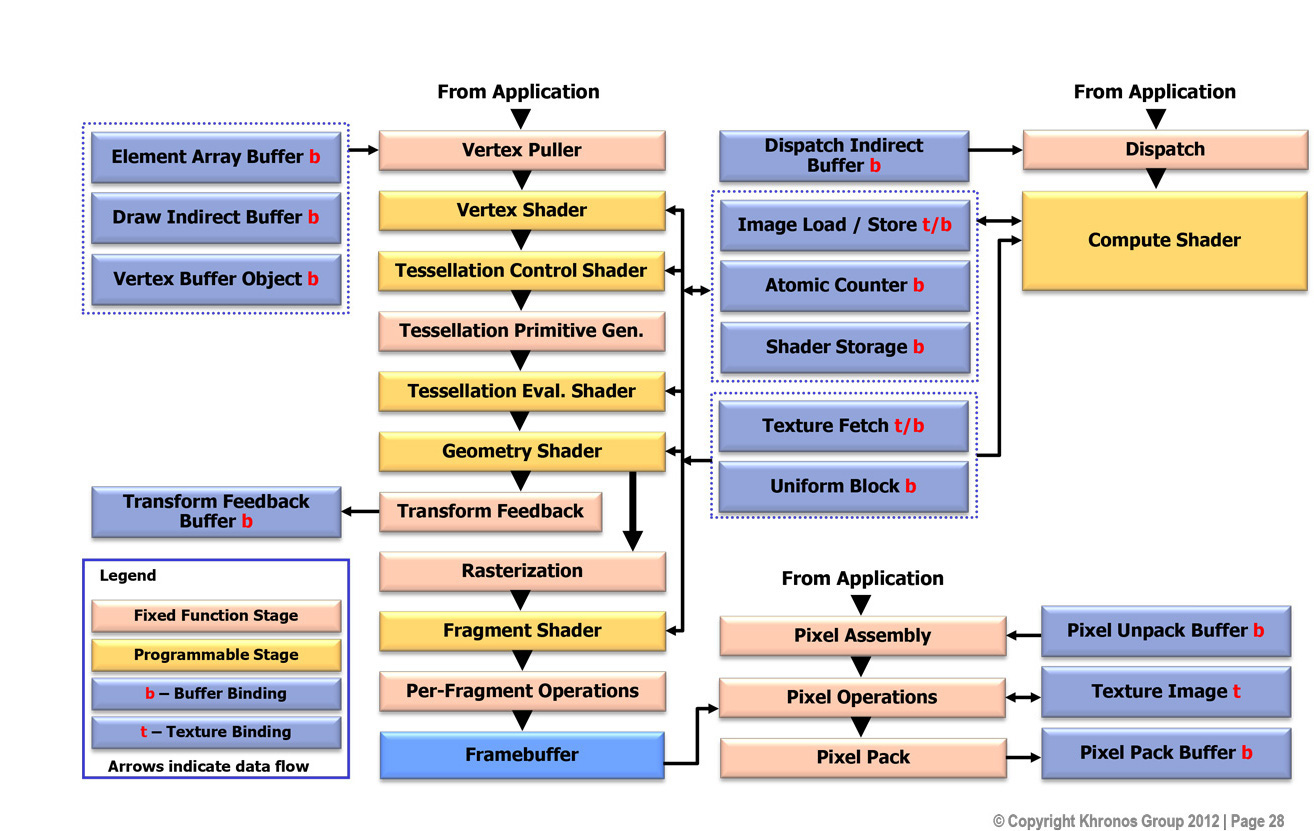
\includegraphics[width=1\textwidth]{figuras/pipeline.jpg}
    \caption{\textit{Pipeline} do OpenGL 4.x, por \citep{pipeline}. Todos os passos marcados pela cor amarela podem
    ser reprogramados para serem utilziados por aplicações GPGPU. (Modificada)}
    \label{fig:pipeline}
\end{figure}

\begin{figure}[H]
    \centering
    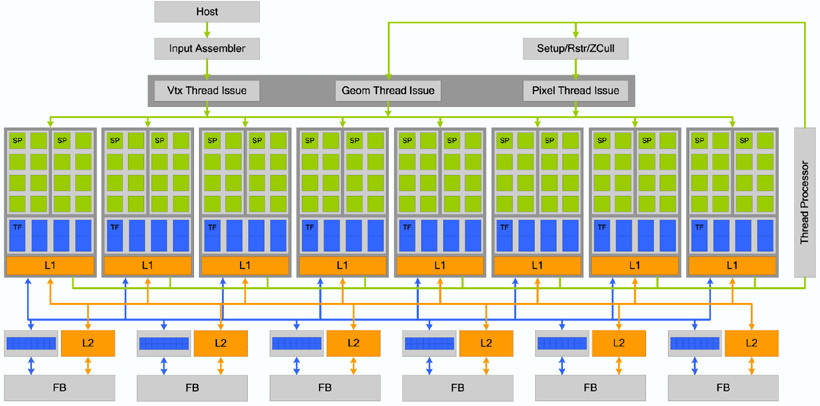
\includegraphics[width=1\textwidth]{figuras/simd.jpg}
    \caption{Arquitetura da GPU SIMD, por \citep{blythe2008rise}.}
    \label{fig:simd}
\end{figure}

\subsection{CUDA}\index{CUDA}
\textit{Compute Unified Device Architecture}, definida pela (CUDA) é uma arquitetura de programação para GPUs criada
pela ~\cite{nvidia2007compute}.
Ele adiciona suas diretrizes para as linguagens C, C++, FORTRAN e Java, permitindo que elas usem a GPU.
Esse trabalho usa o CUDA junto com a linguagem C.
A versão 1.0 do CUDA foi disponibilizada no inicio de 2007. Atualmente só existe um compilador para CUDA, o nvcc,
e ele só da suporte para GPUs NVIDIA.

Para uma função executar na GPU ela precisa ser invocada de um programa da CPU. Chamamos esse programa de \textit{Host}
e a GPU onde o kernel irá executar de \textit{Device}.

O CUDA implementa um conjunto virtual de instruções e memória, tornando os programas retroativos. O compilador
primeiro compila o código em C para um intermediário, chamado de PTX, que depois será convertido em linguagem
de máquina. Na conversão do PTX para linguagem de máquina o compilador verifica quais instruções o \textit{device}
suporta e converte o código para usar as instruções corretas.
Para obter o maior desempenho possível, é importante saber para qual versão o código final será compilado,
pois na passagem do código de uma versão maior para uma menor não existe a garantia que o algoritmo seguira as mesmas instruções,
o compilador pode mudar um conjunto de instruções para outro menos eficiente, ou em alguns casos, algumas instruções não existem em
versões mais antigas do hardware.

\subsubsection{Modelo de Plataforma}
A inicialização dos recursos que o CUDA necessita para a comunicação com a GPU é feita no background da
aplicação no momento da primeira chamada de alguma das diretivas do CUDA. Essa primeira diretiva terá um
tempo maior de execução que chamadas subsequentes a mesma diretiva. Na inicialização o CUDA identifica
os \textit{devices} existentes e escolhe um deles para ser o responsável pelas execuções posteriores.

O próximo passo é a alocação de memória no \textit{device}. As operações de leitura de memória de um kernel são feitas somente
na memória de um \textit{device}. A alocação dessa memória é feita pelo \textit{host}, usando \verb#cudaMalloc()#.
Para copiar a memória do \textit{host} para o \textit{device} ou vice-versa,
\verb#cudaMemcpy()# é usada. Para liberar o espaço alocado após a execução basta usar o \verb#cudaFree()#.
Todas essas diretivas recebem um ponteiro do \textit{host}, usado para o controle sobre qual posição da memória está sendo
operado em cada operação.

O CUDA dá suporte a alocação de vetores em duas ou três dimensões através de: \verb#cudaMallocPitch()# e
\verb#cudaMalloc3D()#, respectivamente. É necessário usar as modificações dos comandos \verb#Memcpy# para
duas ou três dimensões também, que são: \verb#cudaMemcpy2D()#, \verb#cudaMemcpy3D()#.

\subsubsection{Modelo de Programação}
Um kernel no CUDA é uma função C que será executada paralelamente $n$ vezes em $n$ \textit{threads} diferentes na GPU. Um kernel pode ser
definido em qualquer lugar do seu código, usando a declaração \verb#__global__# do lado esquerdo do tipo de retorno do kernel.
Para invocar um kernel, o \textit{host} faz a chamada de uma função com a sintaxe parecida com o C, mas usa uma configuração de
execução definida pelo CUDA, que usa a sintaxe \verb#<<<...>>># junto da chamada da função. Os parâmetros da configuração são
o número de blocos de \textit{threads} e o número de \textit{threads} por blocos. Para somar dois vetores de tamanho M e guardar o resultado num
outro vetor, o código é o seguinte:

\begin{lstlisting}
  __global__ void MatrixMulti ( float* a, float* b, float* c) {
    int i = threadIdx.x;
    a[i] = b[i] + c[i];
  }

  int main () {
    ...
    VecAdd<<<1,M>>>(a, b, c)
    ...
  }
\end{lstlisting}

No kernel acima, a linha \verb#int i = threadIdx.x# atribui a variável i o valor do índice da \textit{thread} atual na primeira dimensão.
A estrutura \verb#threadIdx# é um vetor de 3 dimensões, logo as \textit{threads} podem ser organizadas em 1, 2 ou 3 dimensões dentro de um
\textit{device}. As \textit{threads} são organizadas por blocos. Cada bloco tem dimensões maleáveis, mas as GPUs atuais limitam para 1024 o
número máximo de \textit{threads} por blocos. Cada bloco é lançado para execução em um processador diferente. Blocos são organizados em
grids, que tem seu tamanho configurado na chamada o kernel, bem como o tamanho de cada bloco. No nosso exemplo acima, na linha
\verb#VecAdd<<<1,M>>>(a,b,c)#, o 1 determina o número de blocos e o M o número de \textit{threads} por bloco.

O CUDA supõem que todos os blocos podem ser executados de maneira independente, ou seja, eles podem executar tanto paralelamente
quanto sequencialmente. Com isso, é possível que o desempenho do código aumente em GPUs com mais processadores, sem que o programador
tenha que modificar o código.

O CUDA utiliza o Compute Capability (Capacidade Computacional) do \textit{device} no qual ele irá executar o \textit{kernel}
para identificar quais instruções ele pode utilizar. A Compute Capability de um \textit{device} é um número de dois digitos,
um que representa a arquitetura do \textit{device}, e outro que representa melhorias numa arquitetura.
A arquitetura \textit{Tesla}, a primeira da NVIDIA a dar suporte a GPGPU, tem Compute Capability 1.x, a seguinte, a \textit{Tesla},
tem 2.x e a atual, a \textit{Kepler}, tem 3.x. Dentro de cada arquitetura, podem existir melhorias nas instruções, que são
refletidas no número após o ponto, ou seja, uma placa com Compute Capability 2.1 tem instruções que uma 2.0 não tem.

\subsubsection{Hierarquia de Memória}
No CUDA, a memoria é separada logicamente em 4 locais:

\begin{itemize}
  \item Registradores - Toda variável de uma \textit{thread} fica em registradores.
  \item Memória Local - Memória acessível por cada \textit{thread} separadamente, mas de uso pouco provável. Ela só é usada se
          não existe mais espaço nos registradores ou se o compilador não ter certeza sobre o tamanho de um vetor.
  \item Memória Compartilhada - Cada bloco de \textit{threads} tem uma memória compartilhada. A memória compartilhada é separada em
          pequenos blocos independentes. Se uma requisição de leitura tem n endereços em n blocos diferentes, o tempo de leitura
          desses n endereços é igual ao tempo de leitura de 1 endereço. Caso duas leituras caiam no mesmo bloco, elas serão
          feitas sequencialmente. A memória compartilhada fica em chips dentro dos SMs, logo seu acesso é mais rápido do que o acesso a
          memória global.
  \item Memória Global - A memória global é acessível por qualquer bloco em execução em um \textit{device}. A memoria global não é
          apagada após a execução de um kernel, então chamadas subsequentes de um mesmo kernel simplesmente leem os resultados
          da memória global. Existe um pedaço da memória global reservada para valores constantes do programa.
\end{itemize}

Por padrão, o compilador do CUDA cuida do gerenciamento da memória, ou seja, ele é o responsável por distribuir os dados
entre os locais diferentes de memória. O programador pode dar dicas para o compilador usando qualificadores indicando o local
que ele quer que aquele elemento fique na memória. Os possíveis qualificadores são:
\begin{itemize}
  \item \verb#__device__# Fica na memória global.
  \item \verb#__constant__#   Fica na area constante da memória global.
  \item \verb#__shared__# Fica na memória compartilhada das \textit{threads}.
  \item \verb#__restrict__# Indica para o compilador que todos os ponteiros com esse qualificador apontam para locais diferentes
                            da memória. Isso é importante pois o compilador pode fazer otimizações com o código sabendo dessa informação.
\end{itemize}

GPUs com Compute Cabapility maior ou igual a 2.0 podem alocar memória dentro do \textit{device} em tempo de execução.

%% ------------------------------------------------------------------------- %%
%% ------------------------------------------------------------------------- %%
\section{Algoritmos de Registro}\label{sec:algReg}
    Escolhemos dois algoritmos com base na facilidade deles em adotar uma paralelização seguindo o modelo SIMD.
Falaremos mais sobre eles abaixo.

%% ------------------------------------------------------------------------- %%
\subsection{\textit{Demons}}\index{Demons}
    O \textit{Demons} foi proposto por \cite{thirion1995fast}. Diferentemente de grande parte dos algoritmos de registro,
ele não segue exatamente os passos descritos acima. Ele tem como base o modelo de atratores, que dado dois conjuntos de pontos
em cada uma das imagens, os pontos da imagem Alvo são atraídos para seus pares na imagem Referência utilizando alguma métrica.
A métrica mais básica de atração é a de vizinhos próximos, que leva cada ponto ao ponto mais próximo da imagem de
referência, mas técnicas mais elaboradas como a similaridade de curvatura ou intensidade podem ser utilizadas para
aumentar a acurácia. Os pontos da imagem alvo então movimentam a imagem até que eles encontrem algum ponto da imagem
de referência.

    O \textit{Demons} aplica uma dimensão de informação a mais ao modelo de atratores, acrescentando a cada ponto uma direção
associada ao gradiente da imagem. Um exemplo pode ser visto na imagem \ref{fig:demons}.
Chamamos cada um desses pontos de \textit{Demon}. Com essa informação o algoritmo é capaz
de identificar pontos dentro e fora do modelo gerado a partir dos \textit{Demons} e direcionar a força para empurrá-los ou
atraí-los, respectivamente. Para obtermos o melhor resultado possível adotamos um \textit{Demon} por pixel/voxel.

\begin{figure}[H]
    \centering
    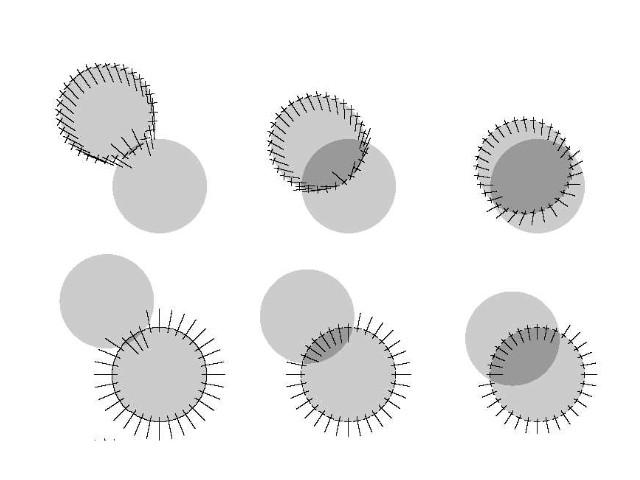
\includegraphics[width=1\textwidth]{figuras/demons.jpg}
    \caption{A primeira linha demonstra o sistema de atratores, enquanto a segunda o Demons, por \citep{thirion1995fast}}
    \label{fig:demons}
\end{figure}

\subsubsection{Aproximação matemática da transformação}
    O \textit{Demons} supõe que a transformação não muda a função de densidade, ou seja, ela só movimenta os pixels e não muda
suas intensidades. A equação seguinte resume isso:
\begin{align}
    i(x(t),y(t),z(t)) = const, \\
\end{align}
    onde $i$ é a intensidade da imagem na posição $x(t),y(t),z(t)$. Derivando (1) temos:
\begin{align}
    \frac{\partial i}{\partial x} \frac{\partial x}{\partial t} +
    \frac{\partial i}{\partial y} \frac{\partial y}{\partial t} = - \frac{\partial i}{\partial t}
\end{align}
    Supondo que as duas imagens que temos diferem de uma unidade de tempo $\partial i/\partial t =
r-a$, \textit{r} e \textit{a} as intensidades de R e A respectivamente e que a velocidade instantânea
$\vec{v} = (dx/dt,dy/dt)$ é aplicada a cada pixel para movê-lo de A para R, chegamos a equação:
\begin{align}
    \vec{v}*\vec{\nabla}r = a - r, \ \text{onde} \ \vec{\nabla} r \ \text{é o gradiente de R}
\end{align}
    O inverso da transformação é aproximado por $\vec{v}$. Porém essa equação é instável em relação a norma de $\nabla
r$. Se a sua norma for muito pequena o \textit{Demon} em questão é levado para o infinito em alguma direção. Podemos levar em
conta a diferença dos pixeis de R e A para normalizar a equação (4), obtendo a forma final do \textit{Demons}:
\begin{equation}
    \vec{v} = \frac{\vec{\nabla}r * (a - r)}{\vec{\nabla}r^2 * (a - r)^2}
\end{equation}

\subsubsection{Implementação}
    Como a formula (5) é degenerada, ou seja, não é possível encontrar uma solução analiticamente para ela,
não podemos calcular o valor de $\vec{v}$ sem utilizar algum artificio. Para tal,
utilizaremos um algoritmo iterativo. Esse algoritmo recebe como entrada as imagens R e A e um campo vetorial
com as dimensões de A que contém uma aproximação da transformação aplicada, esse campo pode ser zero.
Cada iteração realiza 3 passos:
\begin{enumerate}
    \item Para cada \textit{Demon} em $A_i$, calculamos $\vec{v_i}$, criando um novo campo vetorial $V_i$
    \item Aplicamos um filtro Gaussiano para retirar o ruído introduzido pelo processo em $V_i$
    \item Aplicamos $V_i$ em $A$ para obter $A_{i+1}$;
\end{enumerate}
    Esse processo é feito até que $A_i$ convirja à $R$. É importante lembrar que é necessário a
utilização de um algoritmo de interpolação, já que é extremamente provável que o vetor $\vec{v}$
leve os pontos para posições não inteiras. A interpolação trilinear já é suficiente para tal.

\subsubsection{\textit{Demons} Simétrico}\index{Demons Simétrico}
    O método acima é conhecido como \textit{Demons} Assimétrico, pois ele só utiliza informações vindas
da imagem referência. No mesmo artigo, Thirion propõe um outro método, conhecido como Simétrico.
Nele a equação para o cálculo de $\vec{v}$ leva o gradiente das imagens $A_i$. Ele obtém resultados
melhores ao custo do cálculo do gradiente de $A_i$ em toda iteração. Sua fórmula é dada por:
\begin{align}\label{math:demons}
    \vec{v} = \frac{4(a - r)*\vec{\nabla}r|\vec{\nabla}r||\vec{\nabla}a|}
                    {(\vec{\nabla}r+\vec{\nabla}a)^2*(\vec{\nabla}r^2 + \vec{\nabla}a^2 + 2(a - r)^2)}
\end{align}

\subsubsection{Pseudo Algoritmo e Tempo Assintótico de Execução do \textit{Demons} Simétrico}

  Abaixo temos a construção de um pseudo algoritmo do \textit{Demons} Simétrico, e de uma subfunção importante para sua
execução, a \textit{calcularCampoInstantaneo}, que calcula o deslocamento dos \textit{Demons} na iteração atual,
deslocamento esse que será somando ao campo de deslocamento total:

\begin{lstlisting}[mathescape]
demons(imagemReferencia, imagemAlvo, campoDeslocamento):
  gradienteRef <- calcularGradienteDaImagem(imagemReferencia)
  campoInstantaneo = 0
  execute:
    campoInstantaneoAntigo = campoInstantaneo
    imagemEstimada <- aplicarCampoAImagem(campoDeslocamento, imagemAlvo)
    campoInstantaneo <- calcularCampoInstantaneo(gradienteRef, imagemReferencia, imagemEstimada)
    campoInstantaneo = filtroGaussiano(campoInstantaneo)
    campoDeslocamento = campoDeslocamento + campoInstantaneo
  enquanto (campoInstantaneo - campoInstantaneoAntigo) <= $\epsilon$:
\end{lstlisting}

\begin{lstlisting}[mathescape]
calcularCampoInstantaneo(gradienteRef, imagemReferencia, imagemEstimada):
  campoInstantaneo = 0
  para x = 0, x menor que $n_l$ :
    para y = 0, y menor que $n_c$ :
      gradienteEstimado <- calcularGradienteDaImagem(imagemEstimada)
      diff = imagemEstimada[x,y] - imagemReferencia[x,y]
      vetorGradSimetrico = gradienteEstimado[x,y] + gradienteRef[x,y]
      campoInstantaneo[x,y] = $\frac{2*vetorGradSimetrico*diff}{(diff^2+vetorGradSimetrico^2)}$
  return campoInstantaneo
\end{lstlisting}

\begin{lstlisting}[mathescape]
calcularGradienteDaImagem(imagem):
  gradiente = 0
  para x = 0, x menor que $n_l$ :
    para y = 0, y menor que $n_c$ :
      gradienteLinha = $\frac{imagem[x+1,y] - imagem[x-1,y]}{2}$
      gradienteColuna = $\frac{imagem[x+1,y] - imagem[x-1,y]}{2}$
      gradiente[x,y] = {gradienteLinha, gradienteColuna}
  return gradiente
\end{lstlisting}

  As tabelas abaixo mostram o tempo de execução assintótico do \textit{Demons} Simétrico, totalizando
$\mathcal{O}(x*n_l^2*n_c^2)$:

\begin{table}[H]
\begin{center}
\begin{tabular}{l|c}
\hline
Tempo de execução do algoritmo \textit{Demons} Simétrico \\
\hline
Linha&Tempo\\
\hline
2       &$\mathcal{O}(n_l*n_c)$ \\
3       &$\mathcal{O}(1)$\\
4       &$\mathcal{O}(1)$\\
5       &$\mathcal{O}(1)$\\
6       &$\mathcal{O}(n_l*n_c)$\\
7       &$\mathcal{O}(n_l^2*n_c^2)$\\
8       &$\mathcal{O}(n_l*n_c)$\\
9       &$\mathcal{O}(1)$\\
10       &$\mathcal{O}(x)$\\
\hline
Total   &$\mathcal{O}(x*n_l^2*n_c^2)$\\
\hline
\end{tabular}
\caption{Tempo de execução do algoritmo \textit{Demons} Simétrico}
\label{table:tps}
\end{center}
\end{table}

\begin{table}[H]
\begin{center}
\begin{tabular}{l|c}
\hline
Tempo de execução do algoritmo \textit{calcularCampoInstantaneo} \\
\hline
Linha&Tempo\\
\hline
2       &$\mathcal{O}(1)$ \\
3       &$\mathcal{O}(n_l)$ \\
4       &$\mathcal{O}(n_c)$\\
5       &$\mathcal{O}(n_l*n_c)$\\
6       &$\mathcal{O}(1)$\\
7       &$\mathcal{O}(1)$\\
8       &$\mathcal{O}(1)$\\
9       &$\mathcal{O}(1)$\\
\hline
Total   &$\mathcal{O}(n_l^2*n_c^2)$\\
\hline
\end{tabular}
\caption{Tempo de execução do algoritmo \textit{calcularCampoInstantaneo}}
\label{table:interpolar}
\end{center}
\end{table}

\begin{table}[H]
\begin{center}
\begin{tabular}{l|c}
\hline
Tempo de execução do algoritmo \textit{calcularGradienteDaImagem} \\
\hline
Linha&Tempo\\
\hline
2       &$\mathcal{O}(1)$ \\
3       &$\mathcal{O}(n_l)$ \\
4       &$\mathcal{O}(n_c)$\\
5       &$\mathcal{O}(1)$\\
6       &$\mathcal{O}(1)$\\
7       &$\mathcal{O}(1)$\\
8       &$\mathcal{O}(1)$\\
\hline
Total   &$\mathcal{O}(n_l*n_c)$\\
\hline
\end{tabular}
\caption{Tempo de execução do algoritmo \textit{calcularGradienteDaImagem}}
\label{table:interpolar}
\end{center}
\end{table}

\subsubsection{Aceleração do \textit{Demons}}
    O primeiro passo do algoritmo iterativo pode ser acelerado utilizando a arquitetura SIMD. O calculo de um dos vetores
depende do gradiente $\vec{\nabla}r$ e da diferença entre as intensidades da imagem Alvo e Referência $(a - r)$, logo
todos os passos podem ser realizados em paralelo sem perda de desempenho. Tanto a aplicação do filtro gaussiano como
a aplicação do campo vetorial $V$ também podem ser adaptados para a SIMD, pelo mesmo motivo apresentado anteriormente.
Devemos tomar cuidado para garantir que os passos sejam executadas de forma sequencial, ou seja, nenhum pixel deve começar
a execução do passo 2 antes que todos tenham executado o passo 1.

%% ------------------------------------------------------------------------- %%
\subsection{Thin Plate Splines}\index{TPS}
    O Thin Plate Splines (TPS) segue mais rigorosamente os passos gerais de um algoritmo de registro. Ele utiliza
características para criar uma função de interpolação que é utilizada para criar a imagem registrada a partir
da imagem referência. Vários algoritmos podem ser utilizados para adquirir as características que serão usadas
pelo TPS, mas não abordaremos esse assunto pois ele foge do escopo do trabalho. Assumimos no inicio da sua
execução que 2 conjuntos de características existem, um para cada imagem, e que uma correspondência entre
eles já é estabelecida.

    Dados as características na imagem referência $(x_i,y_i, i=1,..,n)$ e na imagem alvo $(X_i,Y_i, i=1,..,n)$
o TPS cria uma função que mapeia exatamente cada característica da imagem referência na sua
correspondente na imagem alvo e que é capaz de interpolar os pontos restantes para a imagem final. Para realizar
essa tarefa é utilizada uma função que define uma superfície que sofre a ação de pesos centrados nas
características da imagem referência. A superfície é definida pela seguinte equação, escrita por \cite{bookstein1989principal}:

\begin{align}\label{math:tps}
    f(x,y) = A_0 + A_1x + A_2y + \sum_{i=0}^n F_i r_i^2 ln r_i^2
\end{align}
Onde $r_i^2 = (x-x_i)^2 + (y-y_i)^2 + d^2$, $d$ é um fator de rigidez da superfície, quanto mais próximo de
zero $d$ é mais a superfície sofre ação dos pontos de controle, e os pontos $(x_i, y_i)$ são os pontos de controle.

    O TPS deve então determinar os valores das variáveis $A_0, A_1, A_2$ e dos $F_i$.
Isso é feito através do sistema linear:

\begin{align}
\begin{split}
    \sum_{i=1}^n F_i &= 0 \\
    \sum_{i=1}^n F_ix &= 0 \\
    \sum_{i=1}^n F_iy &= 0 \\
    f(x_1,y_1) &= A_0 + A_1x + A_2y + \sum_{i=0}^n F_i r_{i1}^2 ln r_{i1}^2 \\
    \vdots \\
    f(x_n,y_n) &= A_0 + A_1x + A_2y + \sum_{i=0}^n F_i r_{in}^2 ln r_{in}^2
\end{split}
\end{align}

A equação $\sum_{i=1}^n F_i = 0$ faz com que a soma dos pesos aplicados a superfície seja zero, fazendo com que
ele não se mova. As equações $\sum_{i=1}^n F_ix = 0$ e $\sum_{i=1}^n F_iy = 0$ garantem que a superfície não vai girar.

    Esse sistema deve ser resolvido duas vezes, uma para $f(x,y) = X$ e outra para $g(x,y) = Y$. Com todas as variáveis
encontradas, podemos aplicar as funções de interpolação para desenhar a imagem final.

\subsubsection{Pseudo Algoritmo e Tempo Assintótico de Execução}

  Abaixo temos a construção de um pseudo algoritmo do tps, e de uma subfunção importante para sua execução, a
\textit{interpolar}, que realiza a interpolação da imagem Alvo na construção da imagem registrada:

\begin{lstlisting}[mathescape]
tps(imagemReferencia, imagemAlvo, caracImagemRef, caracImagemAlvo):
  solucaoDaEquLinearEmX <- resolverEquLinear(caracImagemRef, caracImagemAlvo)
  solucaoDaEquLinearEmY <- resolverEquLinear(caracImagemRef, caracImagemAlvo)
  para x = 0, x menor que $n_l$ :
    para y = 0, y menor que $n_c$ :
      novoPontoX <- interpolar(x,y, solucaoDaEquLinearEmX, caracImagemRef)
      novoPontoY <- interpolar(x,y, solucaoDaEquLinearEmY, caracImagemRef)
      novaImagem[x, y] = imagemAlvo[novoPontoX, novoPontoY]
\end{lstlisting}

\begin{lstlisting}[mathescape]
interpolar(x, y, solucaoDaEquLinear, caracImagemRef):
  v[0] = 1
  v[1] = x
  v[2] = y
  para n = 0, n menor que $n_{cp}$ :
    xi = caracImagemRef[n].x
    yi = caracImagemRef[n].y
    r = $\sqrt{(x-xi)^2 + (y-yi)^2}$
    v[n+3] = $r*\log{r}$
  return $v \cdot solucaoDaEquLinear$
\end{lstlisting}

  As tabelas abaixo mostram o tempo de execução assintótico do tps, totalizando
$\mathcal{O}(\frac{4}{3}n_{cp}^3+n_l*n_c*n_{cp})$:

\begin{table}[H]
\begin{center}
\begin{tabular}{l|c}
\hline
Tempo de execução do algoritmo \textit{tps} \\
\hline
Linha&Tempo\\
\hline
2       &$\mathcal{O}(\frac{2}{3}n_{cp}^3)$\\
3       &$\mathcal{O}(\frac{2}{3}n_{cp}^3)$\\
4       &$\mathcal{O}(n_l)$\\
5       &$\mathcal{O}(n_c)$\\
6       &$\mathcal{O}(n_{cp})$\\
7       &$\mathcal{O}(n_{cp})$\\
8       &$\mathcal{O}(1)$\\
\hline
Total   &$\mathcal{O}(\frac{4}{3}n_{cp}^3+n_l*n_c*n_{cp})$\\
\hline
\end{tabular}
\caption{Tempo de execução do algoritmo \textit{tps}}
\label{table:tps}
\end{center}
\end{table}

  O tempo de execução da resolução do sistema linear foi retirada do livro escrito por
\cite[Part~IV]{trefethen1997numerical}, assumindo uma fatoração LU da matriz.

\begin{table}[H]
\begin{center}
\begin{tabular}{l|c}
\hline
Tempo de execução do algoritmo \textit{interpolar} \\
\hline
Linha&Tempo\\
\hline
2       &$\mathcal{O}(1)$ \\
3       &$\mathcal{O}(1)$ \\
4       &$\mathcal{O}(1)$\\
5       &$\mathcal{O}(n_{cp})$\\
6       &$\mathcal{O}(1)$\\
7       &$\mathcal{O}(1)$\\
8       &$\mathcal{O}(1)$\\
9       &$\mathcal{O}(1)$\\
10      &$\mathcal{O}(n_{cp}+3)$\\
\hline
Total   &$\mathcal{O}(n_{cp})$\\
\hline
\end{tabular}
\caption{Tempo de execução do algoritmo \textit{interpolar}}
\label{table:interpolar}
\end{center}
\end{table}

\subsubsection{Aceleração do Thin Plate Splines}

    O primeiro passo para acelerar o TPS é utilizar algoritmos para resolver o sistema linear diretamente na GPU, o que
não é difícil dado que a matriz que representa o sistema sempre é simétrica com uma diagonal de zeros por construção. O
próximo passo para realizar a aceleração do TPS é criar dois vetores que guardam todos os valores possíveis de $(x-x^i)^2$
e $(y-y^i)^2$. O uso desses vetores diminui o número de operações necessárias de $n_l*n_c*n_{cp}$ para $(n_l+n_c)*n_{cp}$.
Da maneira original, a operação $(x-x^i)^2$ é repetida $n_c$ vezes para cada coluna, já com o uso dos vetores esse valor
é calculado uma única vez e acessado toda vez que ele é necessário.

\section{Outros algoritmos de registro estudados}

\subsection{Multiquadrática}
  A função utilizada por esse método de registro pertence a mesma familia do TPS, as funções de interpolação radial.
Elas podem ser definidas, basicamente, pela seguinte fórmula:

\begin{align}\label{math:multiquadric}
    f(x,y) = \sum_{i=0}^n F_i R_i(x,y)
\end{align}

  Quando $R_i(x,y) = \sqrt{(x-x_i)^2 + (y-y_i)^2 + d^2}$, a função é chamada de multiquadrática. Todos os outros passos
para o registro nesse caso seguem o TPS, desde a solução do sistema linear utilizando a correspondência entre as
características para encontrar os $F_i$ até a interpolação realizada para registrar a imagem Alvo. Como reportado
no livro escrito por \cite{goshtasby2005} o TPS é mais eficiente que as multiquadráticas quando existe um termo linear
no registro, algo bastante comum em registro.
%Logo esse método não foi estudado mais a fundo.

\subsection{Média Ponderada}
  Esse grupo de funções não realiza uma interpolação exata das características com suas correspondências como o TPS e
a Multiquadrática fazem. Essas transformações aproximam as características utilizando pesos para cada uma delas em
cada pixel da imagem. A função que a define é:

\begin{align}\label{math:multiquadric}
    f(x,y) = \sum_{i=0}^n f_i b_i(x,y) \\
    b_i(x,y) = \frac{R_i(x,y)}{\sum_{i=0}^n R_i(x,y)}
\end{align}

  Onde $R_i$ é uma função radial descrecente. Quando $R_i$ é uma Gaussiana temos:

\begin{align}\label{math:multiquadric}
    R_i(x,y) = \exp{-\frac{(x-x_i)^2 + (y - y_i)^2}{2\sigma_i^2}}
\end{align}

  Neste caso, o registro por Média Ponderada é chamado de Registro por Gaussiana Racional (RaGs). Novamente os estudos
realizados por \cite{goshtasby2005} mostram que os resultados obtidos pelas RaGs são superiores aos comparados com
o TPS e a Multiquadrática quando todas as características tem correspondências e quando nenhuma característica se encontra
fora da imagem. Quando qualquer uma dessas propriedades se perde, o TPS e a multiquadrática obtém resultados superiores.
%Como os métodos de correspondências não garantem $100\%$ de pareamento, esse método não foi escolhido para passar pelos
%testes abaixo.
